\begin{figure}[h!]
    \centering
    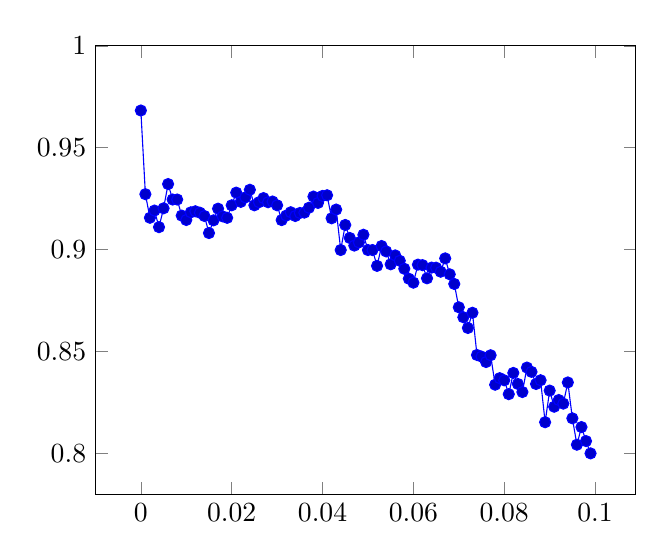
\begin{tikzpicture}
        \begin{axis}[
            legend pos=south west,
            ymax=1,
            xtick={0, 0.02, 0.04, 0.06, 0.08, 0.1},
            xticklabels={0, 0.02, 0.04, 0.06, 0.08, 0.1}
            ]
            \addplot+[sharp plot] coordinates {
            (0.000, 0.968254)
            (0.001, 0.927195)
            (0.002, 0.915612)
            (0.003, 0.919149)
            (0.004, 0.911017)
            (0.005, 0.920259)
            (0.006, 0.932166)
            (0.007, 0.924569)
            (0.008, 0.924569)
            (0.009, 0.916667)
            (0.010, 0.914530)
            (0.011, 0.918280)
            (0.012, 0.918803)
            (0.013, 0.918103)
            (0.014, 0.916488)
            (0.015, 0.908120)
            (0.016, 0.914347)
            (0.017, 0.920086)
            (0.018, 0.916309)
            (0.019, 0.915584)
            (0.020, 0.921739)
            (0.021, 0.927948)
            (0.022, 0.923414)
            (0.023, 0.925602)
            (0.024, 0.929360)
            (0.025, 0.921739)
            (0.026, 0.923246)
            (0.027, 0.925275)
            (0.028, 0.923246)
            (0.029, 0.923581)
            (0.030, 0.921739)
            (0.031, 0.914474)
            (0.032, 0.916667)
            (0.033, 0.918322)
            (0.034, 0.916484)
            (0.035, 0.917960)
            (0.036, 0.918142)
            (0.037, 0.920530)
            (0.038, 0.926009)
            (0.039, 0.922907)
            (0.040, 0.926339)
            (0.041, 0.926667)
            (0.042, 0.915367)
            (0.043, 0.919643)
            (0.044, 0.899782)
            (0.045, 0.912088)
            (0.046, 0.905702)
            (0.047, 0.901961)
            (0.048, 0.903509)
            (0.049, 0.907285)
            (0.050, 0.899782)
            (0.051, 0.899782)
            (0.052, 0.892009)
            (0.053, 0.901747)
            (0.054, 0.899123)
            (0.055, 0.892779)
            (0.056, 0.897155)
            (0.057, 0.894505)
            (0.058, 0.890591)
            (0.059, 0.885714)
            (0.060, 0.883772)
            (0.061, 0.892617)
            (0.062, 0.892377)
            (0.063, 0.885906)
            (0.064, 0.891156)
            (0.065, 0.891111)
            (0.066, 0.889140)
            (0.067, 0.895692)
            (0.068, 0.887872)
            (0.069, 0.883146)
            (0.070, 0.871681)
            (0.071, 0.866812)
            (0.072, 0.861538)
            (0.073, 0.868996)
            (0.074, 0.848291)
            (0.075, 0.847495)
            (0.076, 0.844828)
            (0.077, 0.848156)
            (0.078, 0.833693)
            (0.079, 0.836910)
            (0.080, 0.835853)
            (0.081, 0.829060)
            (0.082, 0.839479)
            (0.083, 0.834061)
            (0.084, 0.830108)
            (0.085, 0.842105)
            (0.086, 0.840000)
            (0.087, 0.834052)
            (0.088, 0.835886)
            (0.089, 0.815287)
            (0.090, 0.830803)
            (0.091, 0.822894)
            (0.092, 0.826180)
            (0.093, 0.824411)
            (0.094, 0.834802)
            (0.095, 0.817204)
            (0.096, 0.804255)
            (0.097, 0.812903)
            (0.098, 0.806034)
            (0.099, 0.800000)
            };
            %\addlegendentry{Precison}
            %\addplot+[sharp plot] coordinates {
            %};
            %\addlegendentry{Recall}
            %\addplot+[sharp plot] coordinates {
            %};
            %\addlegendentry{Negative Recall}
            %\draw[red,line width=1pt] ({axis cs:0.002,0}|-{rel axis cs:0,1}) -- ({axis cs:0.002,0}|-{rel axis cs:0,0});
        \end{axis}
    \end{tikzpicture}
    \caption{Precision and recall w.r.t. lower threshold (no cap on the upper bound)}
    \label{p:lowerbound}
\end{figure}


